\section{Versuchsaufbau und Versuchsdurchführung}

\begin{flushleft}
    Der Aufbau des Versuchs, zu sehen in Abbildung \ref{Abbildung2}, besteht aus einem Kupfer-Röntgenrohr, einem LiF-Kristall oder einem Plexiglas-Streuer und einem Geiger-Müller-Zählrohr.
    Gesteuert kann die Elektronik des Geräts Manuell oder digital über einem Computer werden. 
    Bei der Steuerung über den Computer muss erst das Programm \textit{measure} gestartet werden und unter dem Menüpunkt \textit{Messgeräte}, \textit{Röntgengerät} ausgewählt.
    Dort können dann die Feineinstellungen wie die \textit{Messart}, der \textit{Drehmodus}, den \textit{Kristallwinkel} und die Integrationszeit vorgenommen werden.
    Wenn die Röntgenröhre manuell bedient werden soll, wird zunächst das \textit{RS232-Kabel} abgezogen und das Gerät auf manuell umgestellt.
    Danach wird über den Einstellknopf \textit{neun} der Kristallwinkel oder die Messzeit eingestellt und mit \textit{Enter} bestätigt.
    Auf der oberen Anzeigeleiste werden die gemessenen Zahlraten letztendlich angezeigt. 
    Die Beschleunigungsspannung beläuft sich bei diesem Versuch auf $35\,\unit{\kilo\volt}$ mit einem dazugehörigen Emissionsstrom von $1\,\unit{\milli\ampere}$.
\end{flushleft}


\begin{figure}[H] 
    \centering
    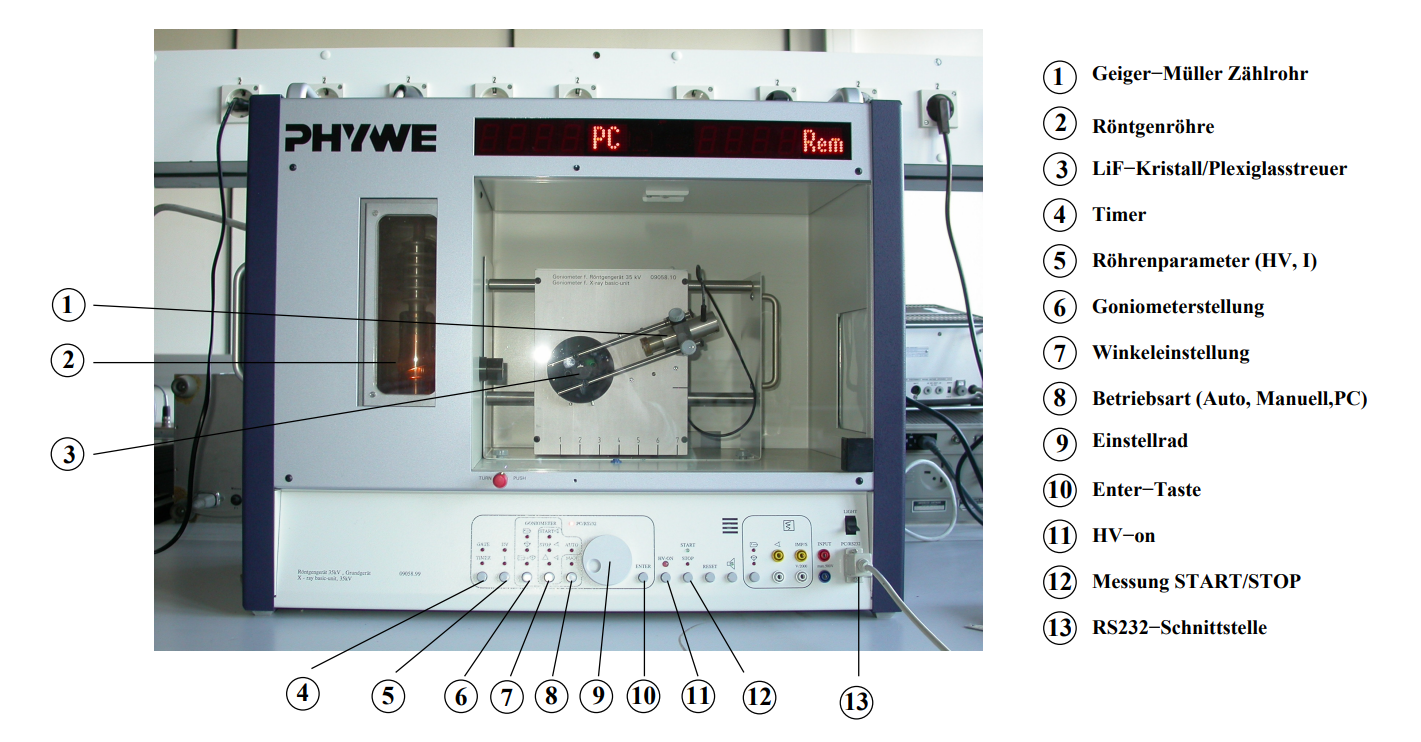
\includegraphics[height=90mm]{bilder/Röntgenröhre.png}
    \caption{Die Abbildung einer Röntgenröhre \cite{a1}.\label{Abbildung2} }
\end{figure}

\subsection{Aufnahme des Emissionsspektrums}

\begin{flushleft}
    Um das Emissionsspektrums aufzunehmen, wird der LiF-Kristall in die Halterung der Röntgenröhre gesteckt und eine $2\,\unit{\milli\meter}$ Blende verwendet.
    Dabei wird die Integrationszeit auf $t=10\unit{\second}$ gesetzt und in einem Winkelbereich von $8\unit{\degree} \leq \alpha \leq 25\unit{\degree} $ in $\increment \lambda = 0.1\unit{\degree}$ Schritten gemessen. 
\end{flushleft}

\subsection{Bestimmung der Wellenlängenabhängigen Transmissionsfunktion}

\begin{flushleft}
    Als Nächstes wird die Zählrate der Röntgenstrahlung mit ($N_{\text{Al}}$) und ohne ($N_{0}$) Aluminium-Absorber auf $t = 200\,\unit{\second}$ gestellt.
    Hierbei geht der gemessene Winkelbereich von $8\unit{\degree} \leq \alpha \leq 25\unit{\degree} $ in $\increment \lambda = 0.1\unit{\degree}$ Schritten gemessen.
    Der Aluminium-Absorber wird dabei vor die $2\,\unit{\milli\meter}$ Blende gesetzt.
    Die Totzeitkorrektur der aufgenommenen Zählrate des Geiger-Müller-Zählrohrs beträgt hierbei $\eta = 90\,\unit{\micro\second}$, wodurch sich im nachfolgenden die Wellenlängenabhängige Funktion der Transmission $T(\lambda)$ aufstellen lässt.    
\end{flushleft}

\subsection{Bestimmung der Compton-Wellenlänge}

\begin{flushleft}
    Bei der Compton-Wellenlängen Bestimmung wird die $2\,\unit{\milli\meter}$ Blende durch eine $5\,\unit{\milli\meter}$ ersetzt und der Lif-Kristall durch ein Plexiglasstreuer ersetzt.
    Die vorher automatische Messung wird auf die manuelle Steuerung gewechselt und der Kristall in einem $45\unit{\degree}$ und $90\unit{\degree}$ Winkel auf das Geiger-Müller-Zählrohr gestellt und die Intensität $I_{0}$ der Kupferröhre gemessen.
    Um dann die Compton-Wellenlänge zu bestimmen, werden zwei unabhängige Messungen durchgeführt.
    Dabei beträgt die Integrationszeit $t=300\,\unit{\second}$. Für die Bestimmung der Transmission $T_{1}$, also die nicht gestreuten Röntgenstrahlen, bestimmt. 
    Danach wird der Aluminium-Absorber in den Strahlengang zwischen Streukörper und Geiger-Müller-Zählrohr platziert und die Transmission $T_{2}$ bestimmt.
    Diese Messungen werden fünf mal wiederholt.
\end{flushleft}
